\chapter{Introduction}
    \section{Terms and Definitions}
    %
        \subsection*{Buoyancy force}\label{sec:Buoyancy force}
        %
            A body submerged in a fluid experiences a force anti-parallel to the gravitational force and proportional to the
            mass of the fluid displaced.
        \subsection*{Surface Tension}
        %
            In a simplified manner attracting intermolecular interactions inside a fluid can be seen as isotrope. Thus,
            they cancel each other out. The closer a particle gets to the interfacing layer of another medium the fewer neighbors
            there are to exert attracting forces from that direction. The attracting force a particle along the interfacing
            layer experiences nets to a force normal to the interface layer and directed inside the fluid.
        %
        \subsection*{Surfactant}
        %
            A material or compound able to alter or even nullify the intermolecular forces inside a fluid (typically a liquid).
        %
        \subsection*{\textsc{Du Noüy}-Method to Measure the Surface Tension of a Liquid}
        %
            A method to measure the surface tension of a liquid by measuring the force withdrawing a submerged ring from that
            liquid \cite{DuNouy.1919.early.ring.method}.
        \subsection*{Other Ways to Measure the Surface Tension of a Liquid}
        %
            \textsc{Andreas-Hauser-Tucker} method or Pendant-drop method: the shape of a droplet is solely dependent of the
            gravitational force and the surface energy. Knowing other parameters of the liquid in question the surface tension
            can be acquired by geometrically evaluating photographs of hanging droplets \cite{Andreas-Hauser-Tucker.surface.tension.pendant.drop.1938}.\par\medskip
            %
            Capillary-tubes method: one opening of a tube of sufficiently small inner diameter is brought in contact with
            the specimen. The liquid will - to some extent - travel along the tube depending on the adhesive forces between
            the liquid and the tube wall, the gravitational force and the cohesive forces along the liquids surface i.e.
            the surface tension.\par\medskip
            %
            Parallel-plates method: similar to the capillary-tubes method, the surface tension can be determined by evaluating
            the rise of the liquid between two parallel plates brought in contact with the liquid.\par\medskip
            %
            Sessile drops and bubbles: in this method, the shape of a drop or bubble resting on a flat and horizontal surface
            is examined.\par\medskip
            %
            \textsc{Jaegers} method: a tube is vertically submerged in a liquid leaving the lower and upper end open. Now,
            if gas pressure is applied to the top of the liquid column inside the tube until a gas bubble escapes the lower
            end the surface tension can be derived from the gas pressure at that moment.\par\medskip
            %
            Oscillating drops and bubbles: much like a pendulum, a drop or bubble is displaced from its shape of equilibrium.
            Released and left alone, it will oscillate about the shape of equilibrium. Measuring the frequency the surface
            tension can be derived \cite{oscillating.drops.surface.tension.Freer.2005}.
        \subsection*{Working Principle of a Strain Gauge}
        %
            Stress induced change of the geometry of a strain gauge translates to a change of its resistance. The impossibility
            to measure electrical resistance directly it typically gets transduced to a voltage signal in order to be further
            processed.
        \subsection*{Working Principle of an Instrumentation Amplifier}
        %
            A instrumentation amplifier is a advanced version of the differential amplifier. A slight variation in the topology
            of the differential amplifier allows to adjust the gain by change of just one resistor. This is beneficial as
            it is likely to introduce distortion changing two resistors while maintaining balance \cite{instrumentation.amp.lessons.electric.circuits.20200216,instrumentation.amp.Kuphaldt.20150217}.
        \subsection*{Resolution of an Analog-Digital Converter}
        %
            An analog-to-digital converter (hereafter referred to as ADC) converts a continuous to a discrete, bitwise signal.
            The number of fractions the ADC is able to divide a given signal to gives the resolution of that ADC.
    \section{Preparation}
    %
        \subsection{Force-Time-Curve}\label{sec:A1 force time curve}% A1
        %
            According to \cref{fig:surface_tension_subdivisions} the force-time-diagram is subdivided into the following 8 parts:
            \begin{enumerate}
                \item The ring is located above the interface. No force is caused.
                \item The ring touches the interface, creating a small positive adhesive force between the ring and the surface.
                \item The ring is about to penetrate the surface while the surface tension creates a small negative force.
                \item The ring is now immersed. Its wires produce a small positive force.
                \item When diving upwards, the force gradually increases.
                \item The ring breaks through the interface and induces an ever-increasing force.
                \item The force reaches its maximum.
                \item The force decreases a bit with the raising until the lamella collapses.
            \end{enumerate}
            \newpage
            \begin{figure}[H]
                \centering
                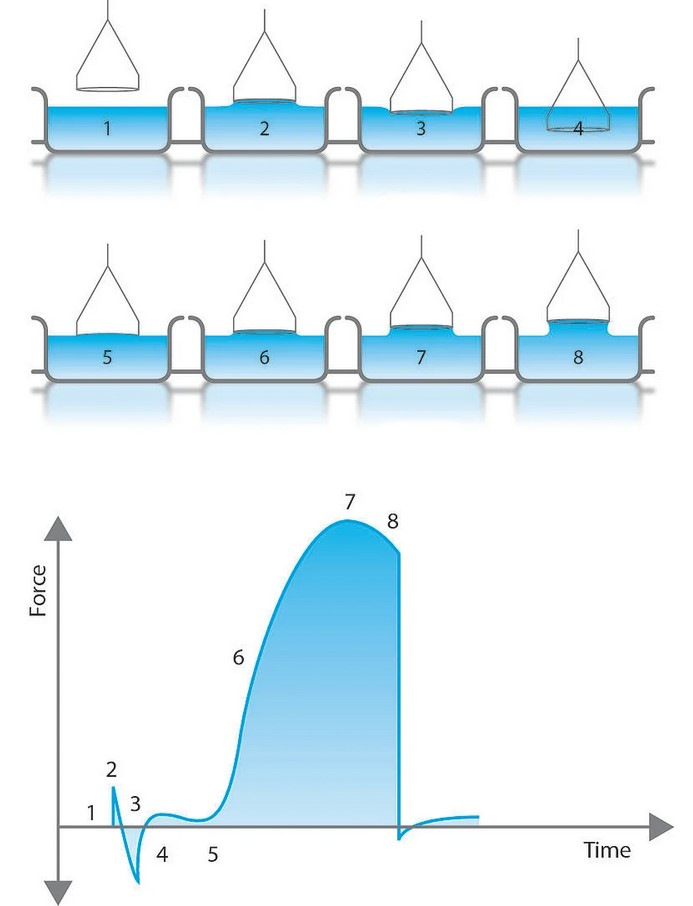
\includegraphics[width=.6\textwidth]{referenzen/surface_tension_subdivisions.jpg}
                \caption[Schematic sequence and curve of the \textsc{Du Noüy} method]{Schematic sequence and curve of the \textsc{Du Noüy} method \cite{Lauren.20210109.3waysMeasureSurfaceTension}.}
                \label{fig:surface_tension_subdivisions}
            \end{figure}
            If the diagram is compared with that in \cref{fig:instructions_fig14}, some differences are noted. For example, there are small
            periodic vibrations that probably have to do with the fluctuation of the ring and other external influences.
            It is particularly noticeable that after penetrating the surface, the force does not rise again into the
            positive, but remains in the negative and only returns into the positive from step 6. Otherwise, from a
            qualitative point of view, everything is similar to that in \cref{fig:surface_tension_subdivisions}, except that after the lamella has
            collapsed, the force oscillates around the zero position.
            %
        \subsection{Surface Tension Formula}\label{sec:A2 derive eq.4}% A2
        %
            The change of area \(\Delta A\) corresponds to the sum of inner and outer radius - \(r_i\) and \(r_o\) respectively - of
            the ring multiplied by the change in height \(\Delta x\):
            \begin{align}
                \Delta A = 2\pi \cdot (r_i + r_o) \cdot \Delta x
                \label{eq:change of area}
            \end{align}
            Since the diameter \(D = 2\bar{r}\) of the ring is much bigger than the thickness \(t = r_o - r_i\), \cref{eq:change of area}
            can be simplified to
            \begin{equation}
                \begin{gathered}
                    2\bar{r} \gg r_o-r_i \quad \Rightarrow \quad r_i \approx r_o \approx \bar{r} \\
                    \Leftrightarrow \\
                    \Delta A = 4\pi \cdot \bar{r} \cdot \Delta x
                    \label{eq:area}
                \end{gathered}
            \end{equation}
            Considering, that the amount of energy \(\Delta E\) is a result of the assumed constant force \(F_0\) multiplied
            by the change in height, it ensues:
            \begin{align}
                \Delta E = F_0 \cdot \Delta x
                \label{eq:energy}
            \end{align}
            Since the surface tension \(\sigma\) is defined as the energy required to increase the surface divided by the change in surface area
            \begin{align}
                \sigma = \frac{\Delta E}{\Delta A}
                \label{eq:surface tension raw}
            \end{align}
            and \cref{eq:area} as well as \cref{eq:energy} are inserted into \cref{eq:surface tension raw}, it follows:
            \begin{align}
                \sigma &= \frac{F_0 \cdot \Delta x}{4\pi \cdot \bar{r} \cdot \Delta x} \nonumber\\
                \sigma &= \frac{F_0}{4\pi \cdot \bar{r}}
                \label{eq:surface tension}
            \end{align}
            %
        \subsection{Gravitational Force of the \textsc{Du Noüy}-Ring in Water and Air}\label{sec:A3 gravi force of du noüy ring}% A3
            %
            Air:

            \begin{equation}
                F_{Ring,Air} = -m_{Ring} \cdot g
            \end{equation}

            Water:

            \begin{align}
                F_{Ring,H_2O}  &= \left( m_{H_2O} - m_{Ring}\right) \cdot g \nonumber \\
                                &= \left(\rho_{H_2O} - \rho_{Al}\right)V_{Ring} \cdot g
            \end{align}
            %
        \subsection{Deriving an Equation for the Bridge Voltage}\label{sec:A4 equation for full bridge circuit}% A4
        %
            \begin{equation}
                U_{Br} = U_2 - U_4 = U_3 - U_1 \quad \text{with} \quad U_{Br} = 0 \text{for} \frac{R_1}{R_2} = \frac{R_3}{R_4}
            \end{equation}
            \begin{equation}
                U_{Br} = U_2 - U_4 = U_0 \cdot \left(\frac{R_2}{R_1 + R_2} - \frac{R_4}{R_3 + R_4}\right)
            \end{equation}
            Defining
            \begin{align}
                R_2 &= R_3 = R + \Delta R \\
                R_1 &= R_4 = R - \Delta R
            \end{align}
            leads to
            \begin{align}
                U_{Br}  &= U_0 \cdot \left(\frac{R + \Delta R}{R - \Delta R + R + \Delta R} - \frac{R - \Delta R}{R + \Delta R + R - \Delta R}\right) \nonumber \\
                        &= U_0 \cdot \left(\frac{R+\Delta R}{2R} + \frac{-R + \Delta R}{2R}\right) \nonumber \\
                        &= U_0 \cdot \frac{\Delta R}{R}
                \label{eq:Ubr and delta R}
            \end{align}
            thus, the bridge voltage is linearly proportional to the factor \( \frac{\Delta R}{R} \).\par
            Now, with the knowledge that the resistance of a body relates with its geometry by
            \( R = \varrho \cdot \frac{l}{b \cdot d} \) and the change of its dimensions under stress follow
            %
            \begin{equation}
                \frac{\Delta b}{b} = -\nu \frac{\Delta l}{l}, \quad \frac{\Delta d}{d} = -\nu \frac{\Delta l}{l}
            \end{equation}
            the bridge voltage can be expressed as
            \begin{align}
                U_{Br} = U_0 \cdot \left( \frac{\Delta \varrho}{\varrho} + \frac{\Delta l}{l} + \nu \cdot \frac{2 \Delta l}{l}\right)
            \end{align}
            %
        \subsection{Schematic Diagram of a Full Bridge}\label{sec:A5 schematic diagram full bridge}% A5
        %
            \begin{figure}[H]
                \centering
                \includesvg[inkscapelatex=false, width=.7\textwidth]{spice/wheatstone/wheatstone.svg}
                \caption[Strain gauge in full bridge configuration]{Strain gauge in full bridge configuration.}
                \label{fig:strain gauge full bridge}
            \end{figure}
        \subsection{Characteristics of HX711}\label{sec:A6 characteristics of the HX711}% A6
        %
            \begin{align}
                &\text{Resolution:}             &&n = \SI{24}{bit}\\
                &\text{Full-scale range:}       &&U_{FSR} = \pm \SI{20}{mV}\\
                &\text{Minimum voltage change:} &&U_{LSB} = U_{FSR} \cdot 2^{-24} \approx \SI{1.2}{nV}
            \end{align}
            %
        \subsection{Impact of Statistical Effects on the effective Resolution}\label{sec:A7 statistical effects}% A7
        %
            The resolution \( n \) of an ADC as per specification implies an ideal, i.e. free-of-noise dc signal. The effective resolution —
            or ENOB (\textbf{E}ffective \textbf{N}umber \textbf{O}f \textbf{B}its) — can be calculated by \cref{eq:ENOB}
            \begin{equation}
                ENOB = n - \log_2{\varsigma}
                \label{eq:ENOB}
            \end{equation}
            where \( \varsigma_{RMS} \) is the RMS (\textbf{R}oot \textbf{M}ean \textbf{S}quare) or standard deviation of the signals noise.
            %
        \subsection{Step Response of an Exponential Filter}\label{sec:A8 step response expo filter}% A8
        %
            \begin{figure}[H]
                \centering
                \includesvg[inkscapelatex=false, width=.9\textwidth]{matlab/step_response/alphas.svg}
                \caption[Exponential filter applied to square step signal]{An exponential filter algorithm applied to a square step signal (light blue) and its responses
                for \(\alpha = 0.5\) (black), \(\alpha = 0.05\) (green) and \(\alpha = 0.01\) (orange).}
                \label{fig:all step response samples}
            \end{figure}
            %
        \subsection{Simulation of the Filter Algorithm}\label{sec:A9 simu of the filter algo}% A9
        %
            \Cref{fig:all expo filtered samples} shows the effect of an exponential filter algorithm applied to a data set to filter
            out statistical noise. The algorithm takes a smoothing factor \(\alpha \in 0 \leq \alpha \leq 1\) as an input and outputs
            a smoothed representation of the raw data.\par 
            \begin{figure}[H]
                \centering
                \subfloat[Expo-smoothing at \(\alpha = 0.01\).\label{subfig:expo alpha 0.01}]{\includesvg[inkscapelatex=false, width=.9\textwidth]{matlab/noisy_data/alpha0.01.svg}}
            \end{figure}
            \begin{figure}[H]\ContinuedFloat
                \centering
                \subfloat[Expo-smoothing at \(\alpha = 0.05\).\label{subfig:expo alpha 0.05}]{\includesvg[inkscapelatex=false, width=.9\textwidth]{matlab/noisy_data/alpha0.05.svg}}
            \end{figure}
            \begin{figure}[H]\ContinuedFloat
                \centering
                \subfloat[Expo-smoothing at \(\alpha = 0.5\).\label{subfig:expo alpha 0.5}]{\includesvg[inkscapelatex=false, width=.9\textwidth]{matlab/noisy_data/alpha0.5.svg}}
                \caption[Examples of an exponential filter algorithm applied to a noisy set of data]{Examples of an exponential
                filter algorithm applied to a noisy set of data. To emphasize its effect on the output, three different values for the smoothing factor \(\alpha\) are shown.
                The raw data is shown in light blue whereas black represents the filtered data. Raw data is provided by Goddard Institute for Space Studies \cite{GISS.nasa.surface.temperature.analysis.20210120}}
                \label{fig:all expo filtered samples}
            \end{figure}
            As seen in \cref{subfig:expo alpha 0.01} a too aggressive filtering of the data could bias the trending of the output
            with respect to the raw data. Too less of smoothing on the other hand might still output too much noise (cf. \cref{subfig:expo alpha 0.5}).
            Depending on the data in question, the smoothing factor needs to be adjusted as needed.
            %
        \subsection{Expected Forces}\label{sec:A10 expected forces}% A10
        %
        Relocating \cref{eq:surface tension} by the force \(F_0\) and knowing the parameters \(\bar{r}\) and \(\sigma\) allows
        for an estimation of that force.\par
        With a radius \(\bar{r} = \SI{0.03}{m}\) and the surface tension of water at room temperature \(\sigma_{H_2O,25} \approx \SI{72}{\frac{mN}{m}}\) \cite{surface.tension.of.pure.water.Pallas.Harrison.1990}
        the force required to tear the lamella calculates to
        \begin{align}
            F_{H_2O,25} &= \sigma_{H_2O,25} \cdot 4\pi \cdot \bar{r} \nonumber \\
                        &= \SI{72}{\frac{mN}{m}} \cdot 4\pi \cdot \SI{0.03}{m} \nonumber \\
                        &\approx \SI{27.1}{mN}
			\label{eq:calculated force}
        \end{align}
